Defintion of the process. \\
Explaining the various contributions. \\
Show few Feynman diagrams and explain that it possesses also tri-boson contribuitions in the s-channel. \\

% \subsection{Scan in $M_{jj}$ and $\Delta y_{jj}$: fiducial region}\label{subsec:scan_full}

\begin{figure}[hbt]
\centering
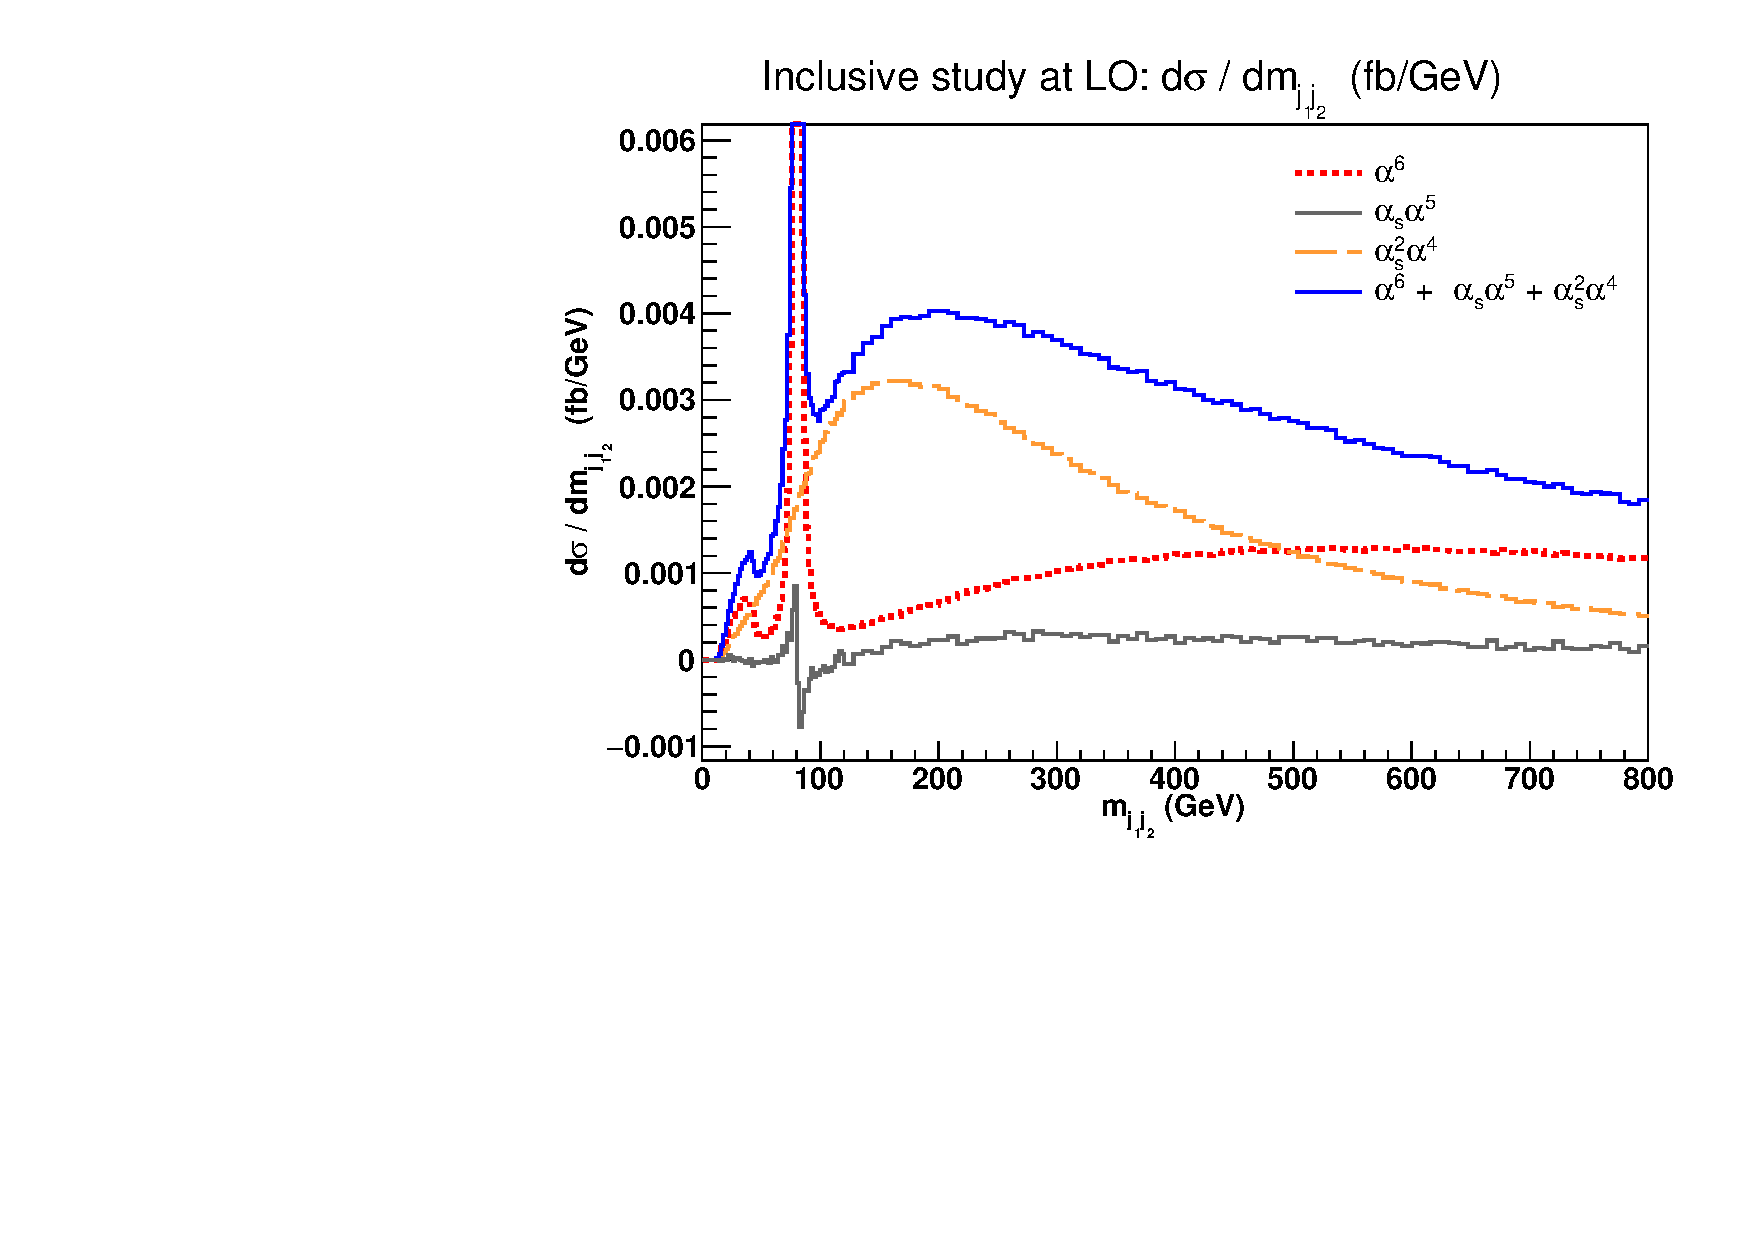
\includegraphics[scale=0.395]{figures/scanfigures/mjj_full.pdf}
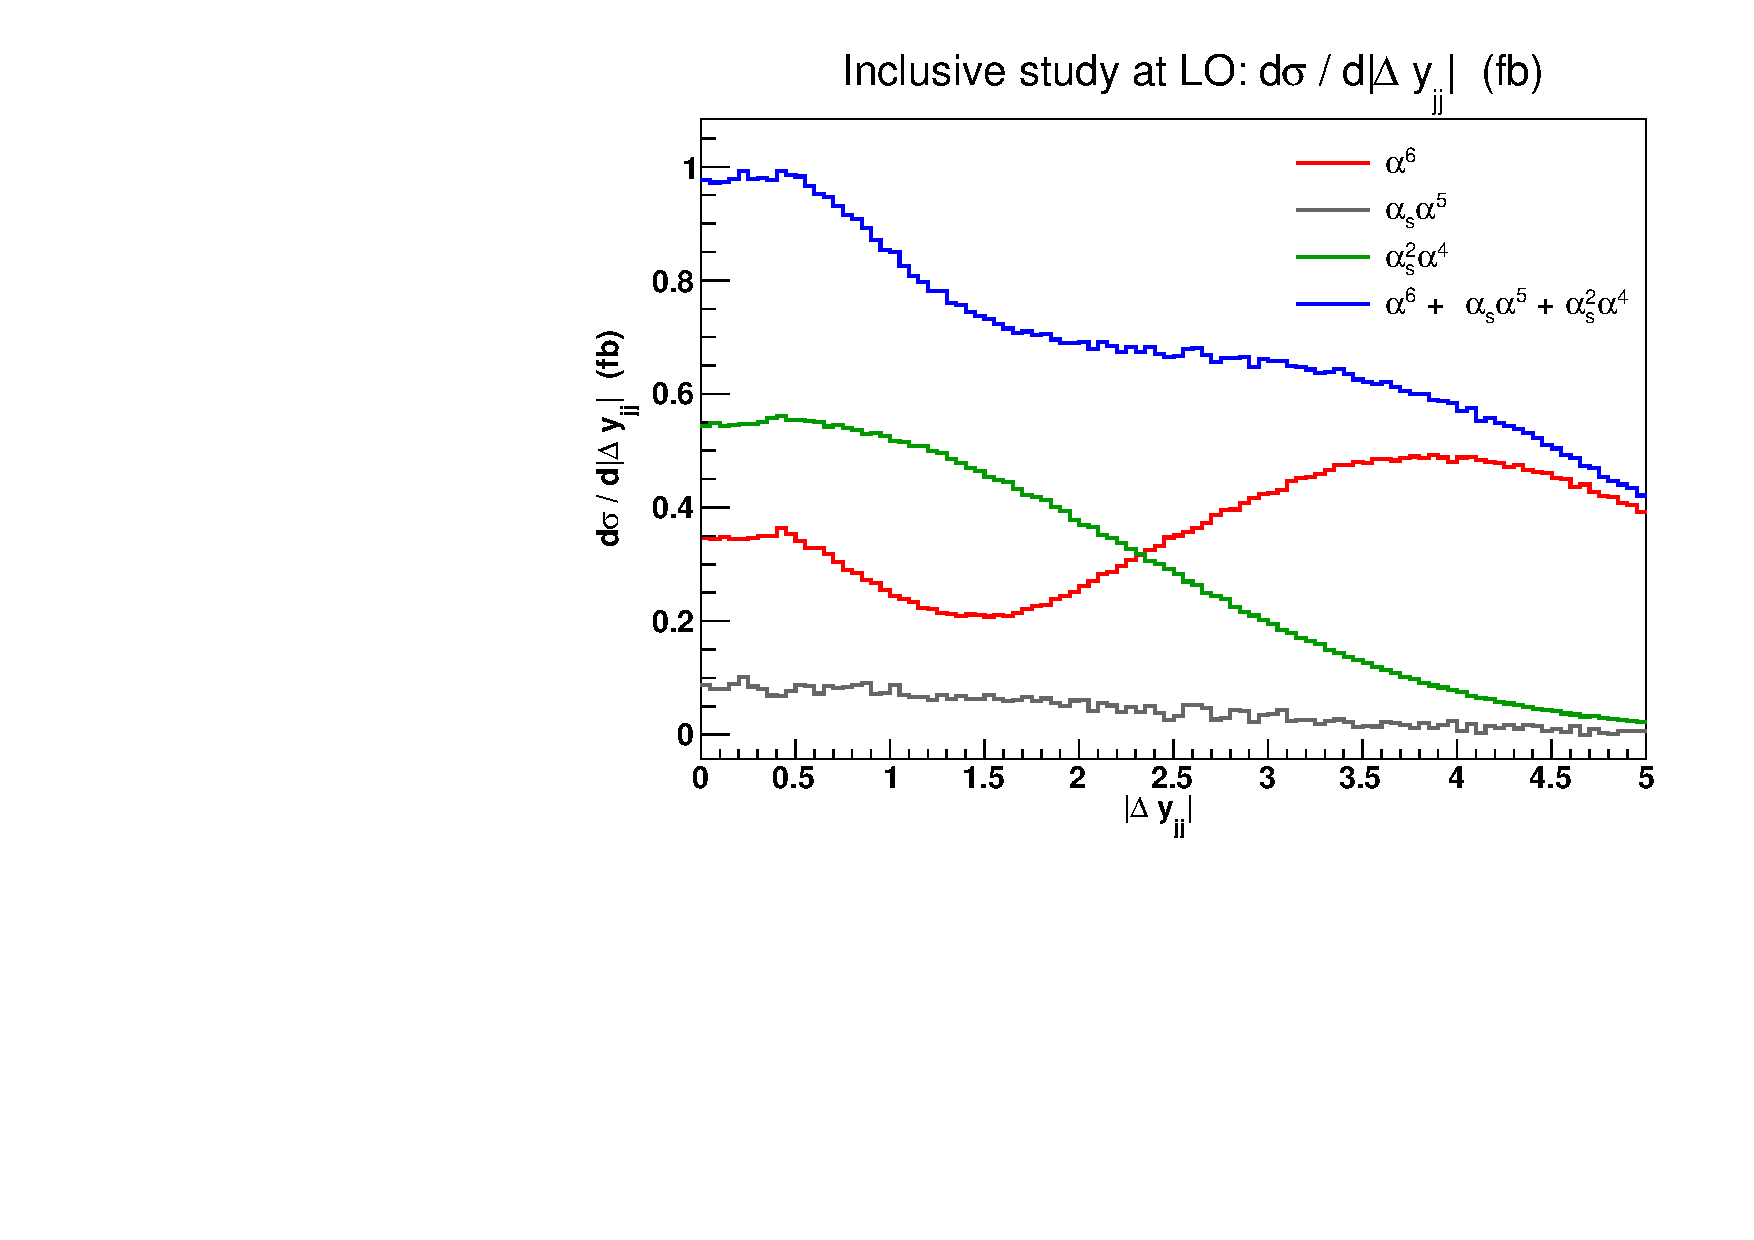
\includegraphics[scale=0.395]{figures/scanfigures/dyjj_full.pdf}
\caption{Differential cross--sections (fb) in $M_{jj}$ (left) and $\Delta y_{jj}$ (right) for the leading perturbative orders, without any cut on the $jj$ pair kinematics. Results of full matrix element \texttt{PHANTOM} calculations.} \label{fig:mjjdyjj_1d}
\end{figure}

\begin{figure}[hbt]
\centering %jjpeak_diag
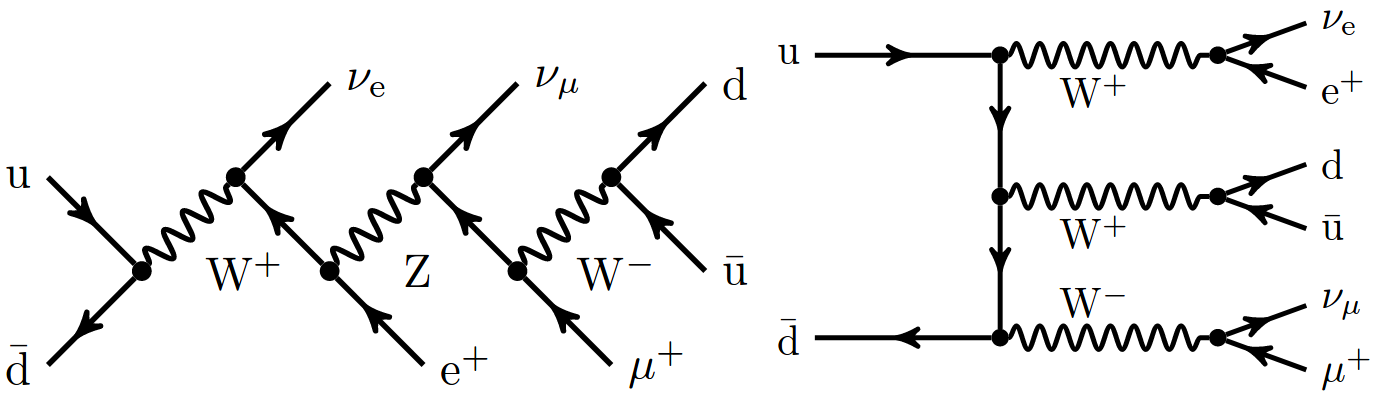
\includegraphics[scale=0.19]{figures/scanfigures/jjpeak_diag.png}
\caption{Tree--level $\mathcal{O}(\alpha_{ew}^6)$ diagrams involving a $W^-$ boson decaying into a $q\bar{q}'$ pair.} \label{fig:jjpeak_diag}
\end{figure}


\begin{figure}[ht]
\centering
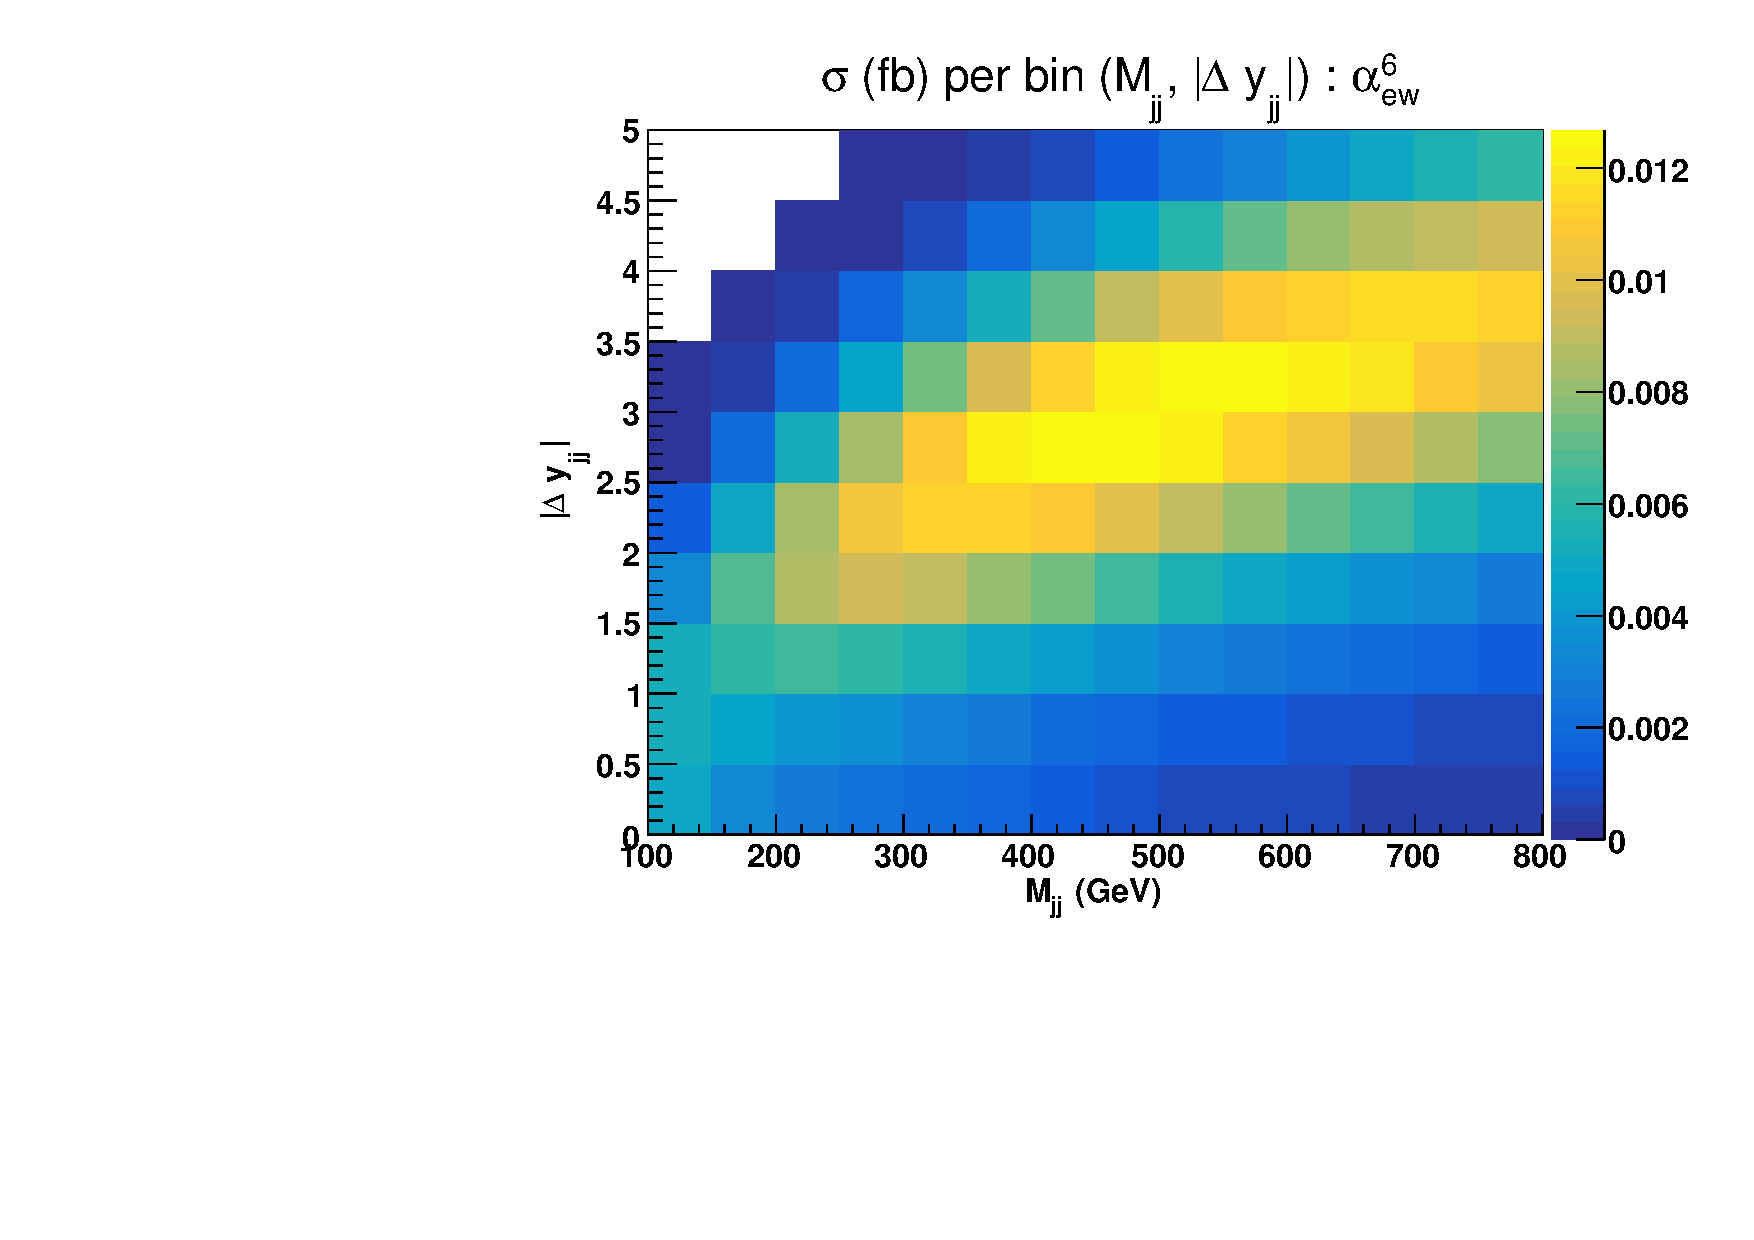
\includegraphics[scale=0.395]{figures/scanfigures/scan_ew6.pdf}
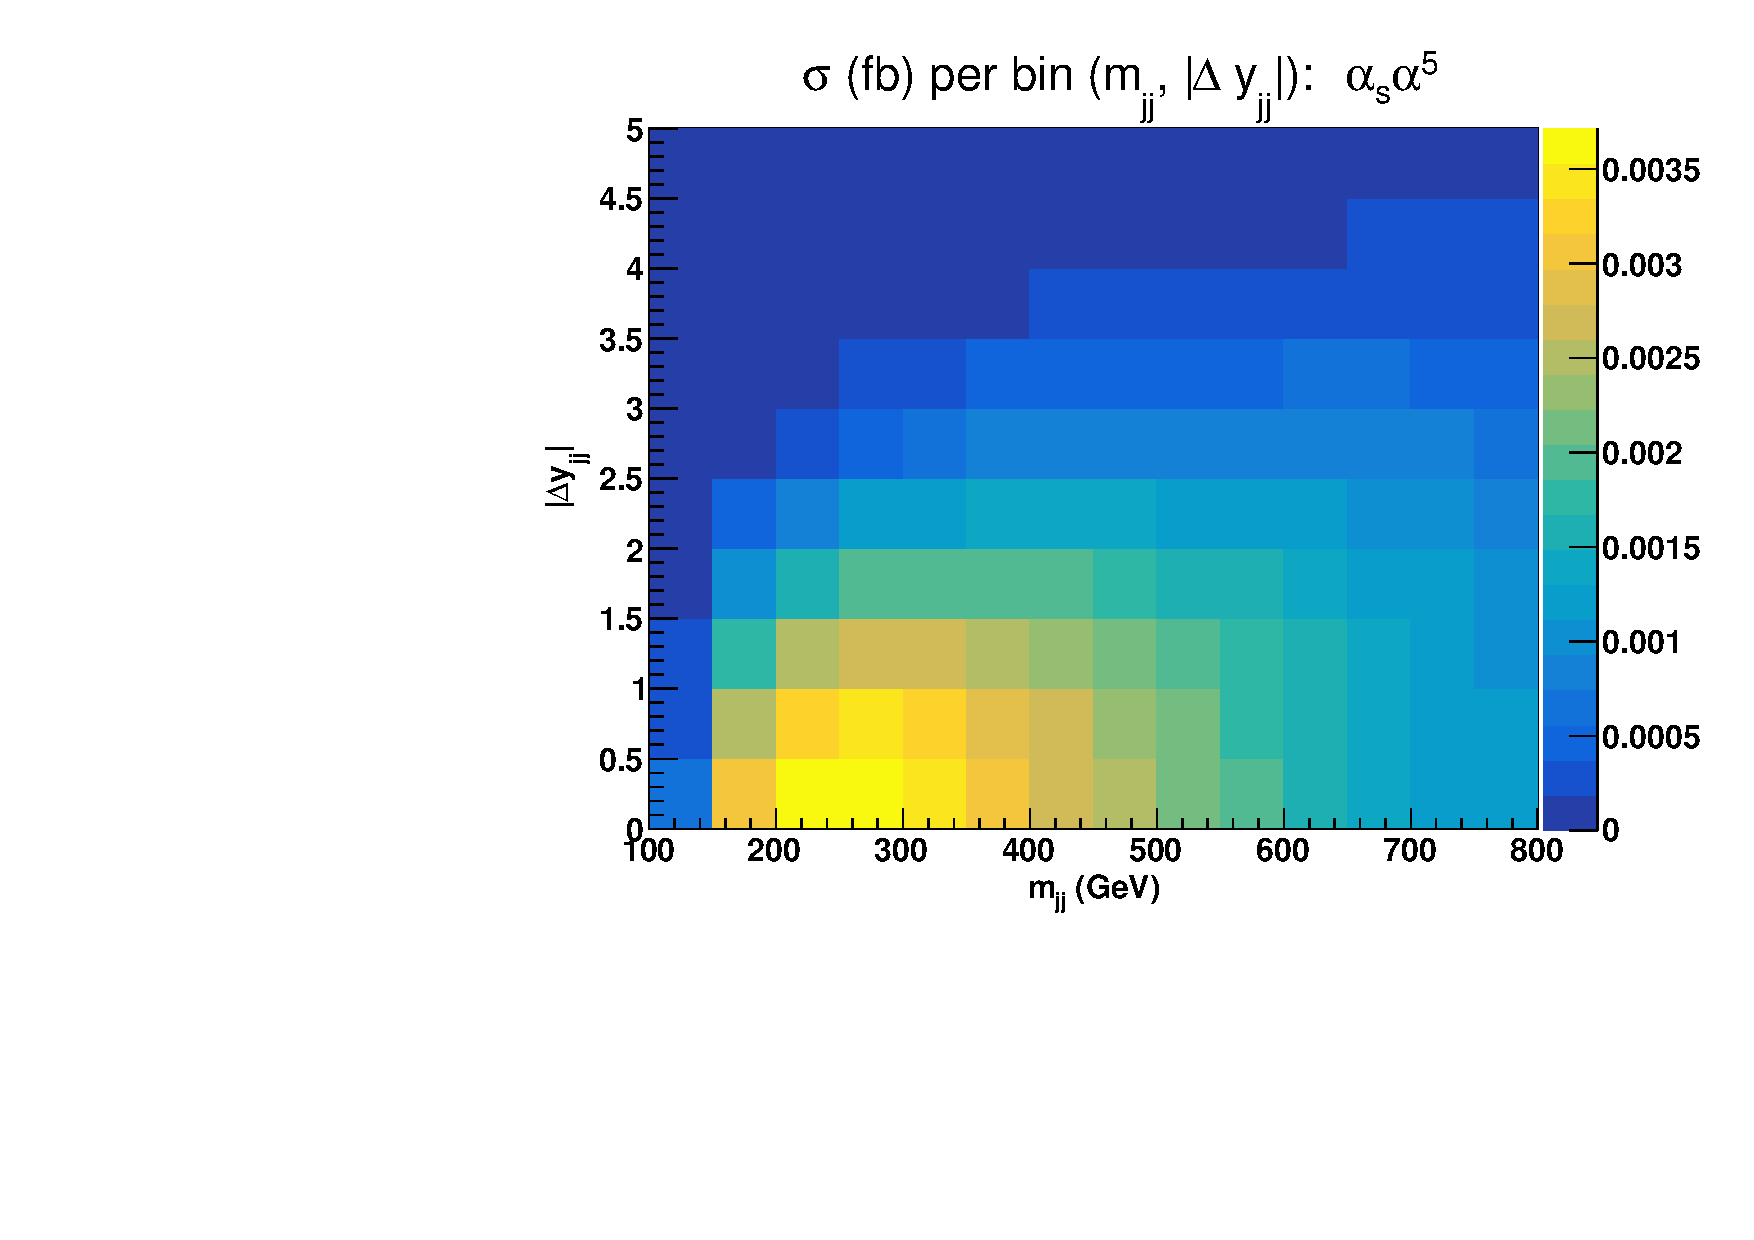
\includegraphics[scale=0.395]{figures/scanfigures/scan_ew5qcd1.pdf}
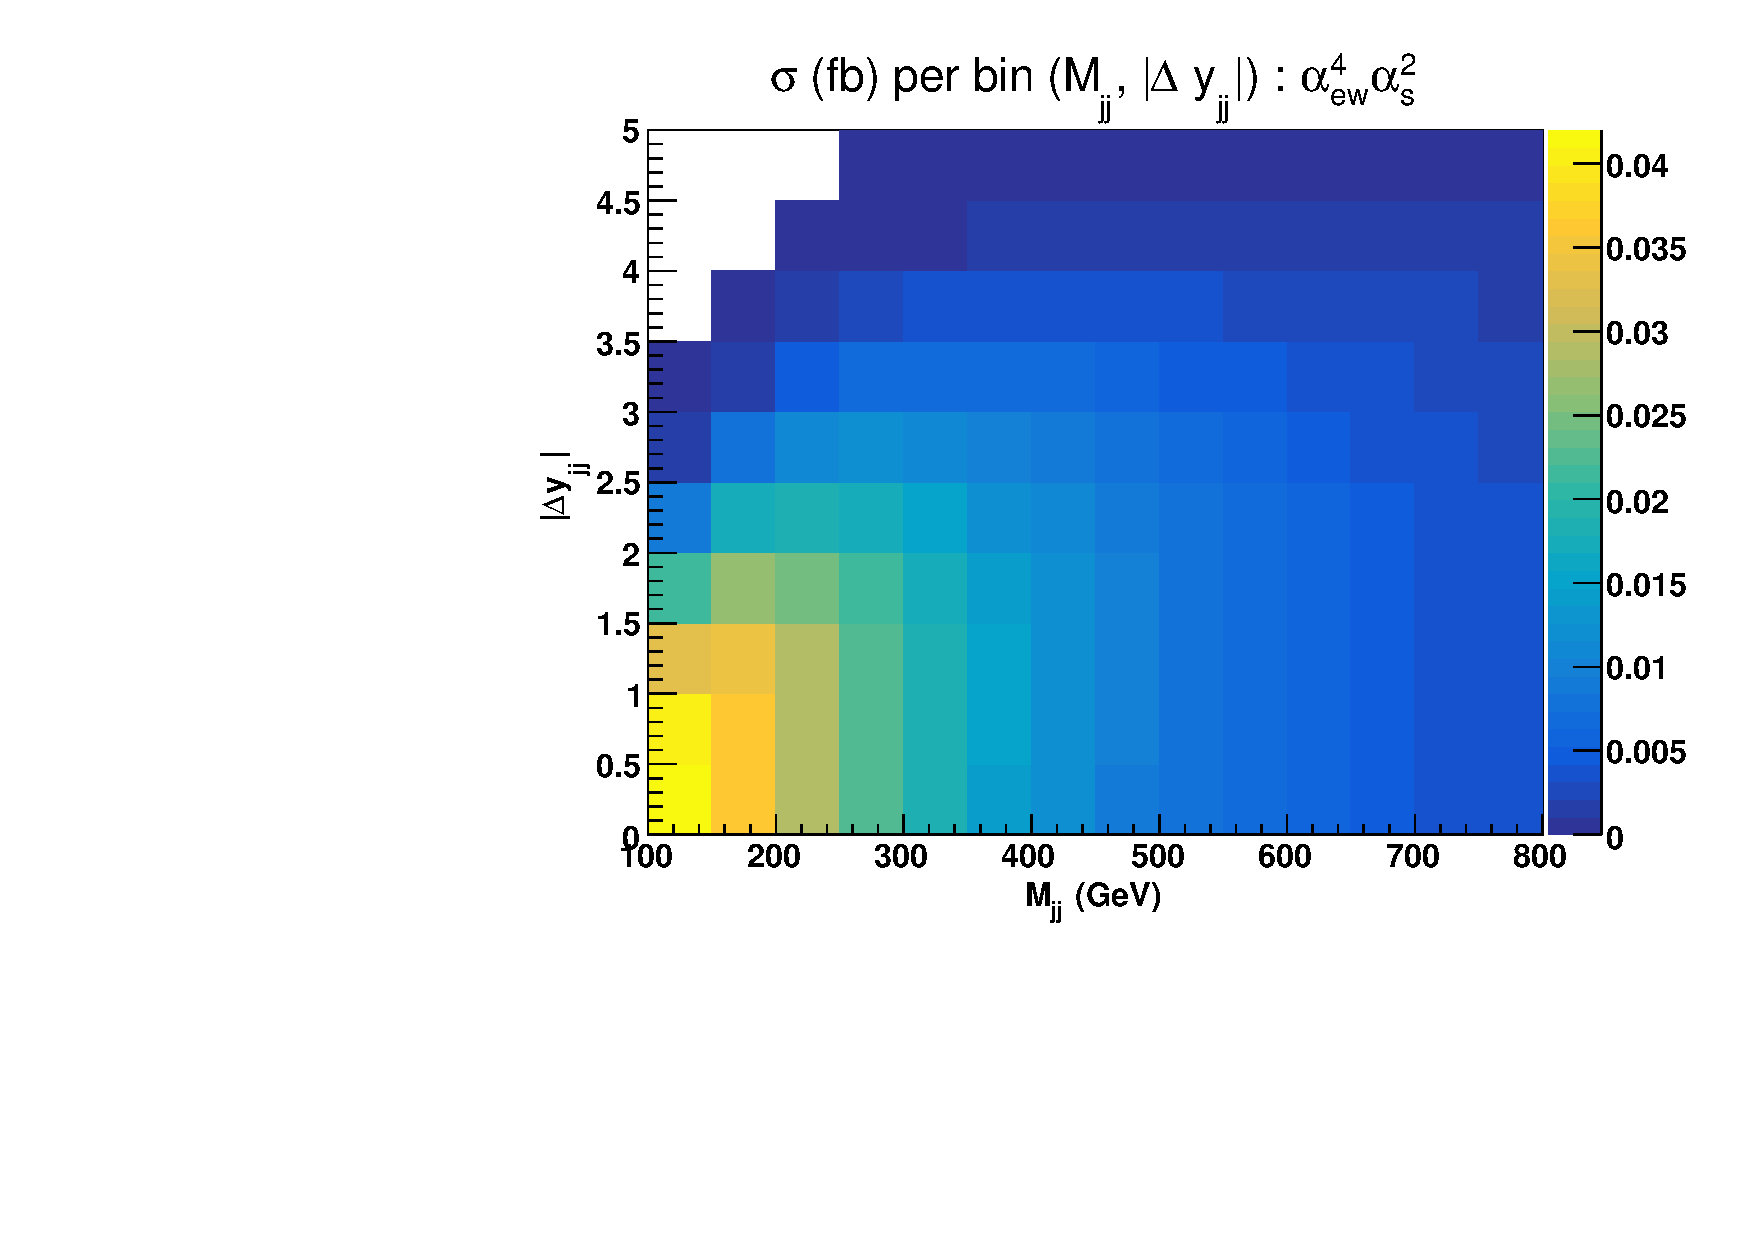
\includegraphics[scale=0.395]{figures/scanfigures/scan_ew4qcd2.pdf}
\caption{Cross--sections (fb) per bin of $(M_{jj},\,\Delta y_{jj})$ at the three leading perturbative orders $\mathcal{O}(\alpha_{ew}^6)$, $\mathcal{O}(\alpha_{ew}^5\alpha_s)$ and $\mathcal{O}(\alpha_{ew}^4 \alpha_s^2)$, without any cut on the $jj$ pair kinematics. Results of full matrix element \texttt{RECOLA} calculations.}\label{fig:mjjdyjj_2d_LO}
\end{figure}
